\chapter{Dataset}
\label{chapter:dataset}
In total,  MDDr. Tichy and his team created two datasets. One dataset was used to detect dental caries and the other for semantic segmentation of dental restorations. The majority of work was done on the first-mentioned set of data.

\begin{figure}
    \centering
    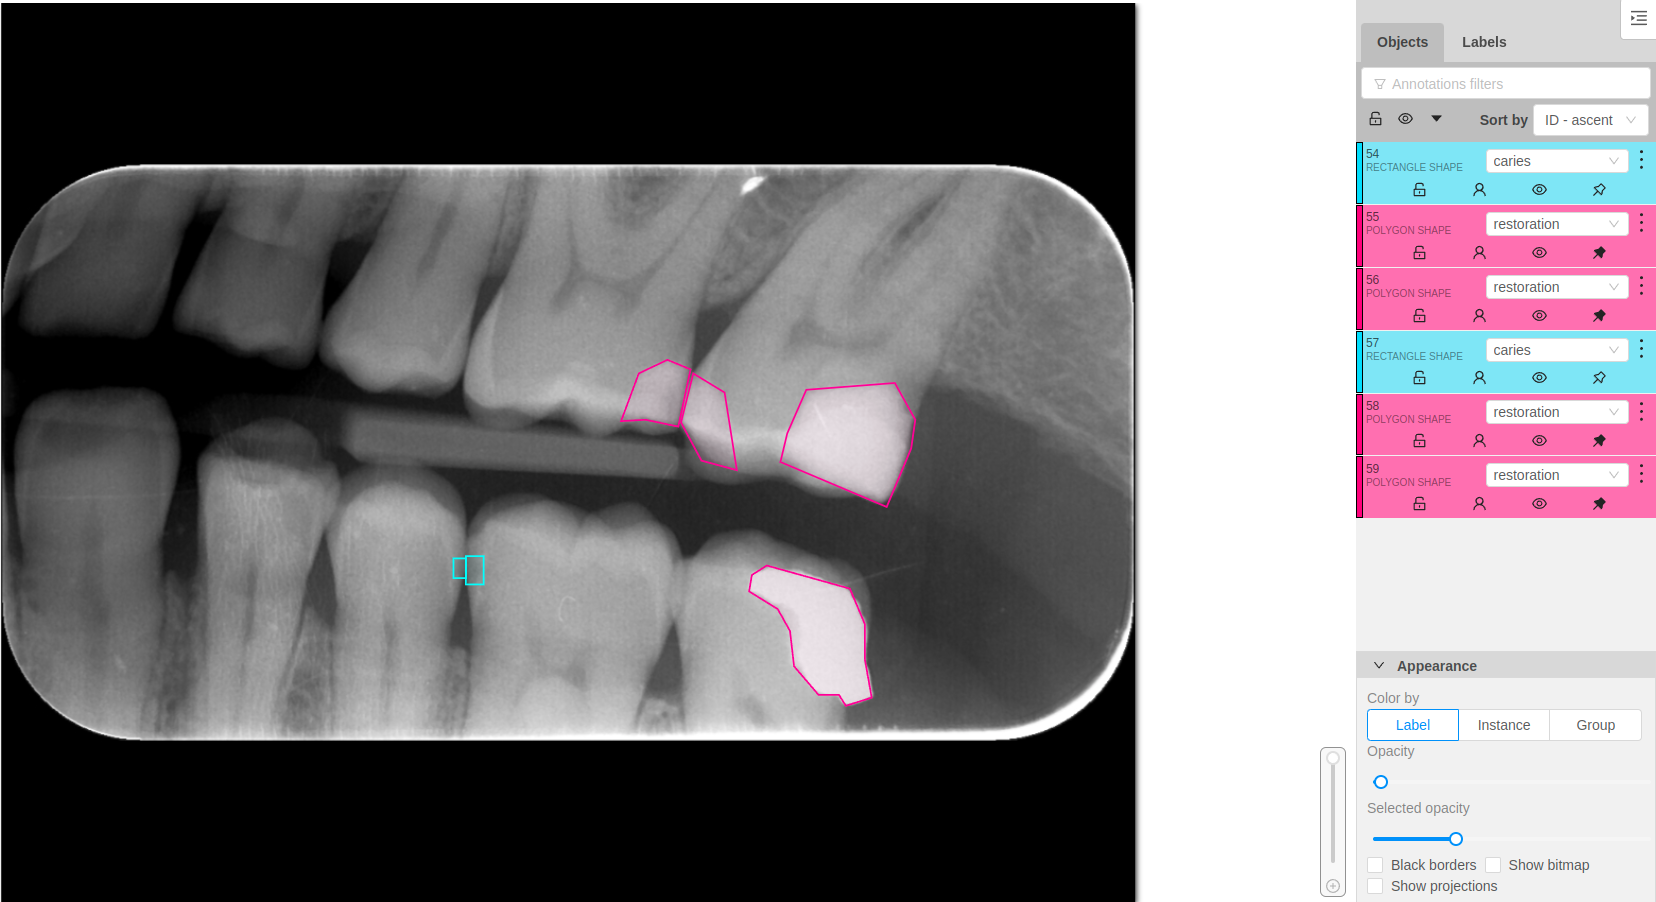
\includegraphics[width=\linewidth]{images/cvat.png}
    \caption{The environment of CVAT with annotated carious lesion and dental restorations}
    \label{fig:cvat}
\end{figure}

\section{Dental caries}
\label{sec:dataset:dental_caries}
MDDr. Tichy and his team began to work on the datasets in September of 2021, along with the beginning of work on this thesis. This led to an opportunity to discuss the format of the data. We decided to annotate every dental caries lesion with a minimal bounding box. The annotation process was conducted in the Computer Vision Annotation Tool (CVAT), running on the Faculty of biomedical informatics server. The web address is www.gdiag.fbmi.cvut.cz.

While denoting the position of the carious lesion, the annotator tried to be consistent with the following guidelines:

\begin{itemize}
    \item Carious lesion is denoted by a rectangle. The rectangle should contain the entire lesion while being as small as possible.
    \item When the lesion is on the proximal surface, and booth teeth are infected, draw a separate box for each of them.
\end{itemize}

Due to constant work on the dataset, we decided to use the same data as long as there was no major update. This ensured that we were able to compare the performance of our models to each other until a significant update was released. In total, six major releases were done. We call these releases the stages of the dataset.

\subsubsection{First stage}
\label{sec:dataset:first_stage}
In the very first stage MDDr. Tichý instructed a group of general dentistry students on how to approach the annotation to get as homogenous dataset as possible. They then annotated a couple of images under his supervision before continuing independently.
Dental X-ray images were uploaded into CVAT and divided into multiple projects, where each project contained between 400-800 images. This was essential due to technical limitations regarding exporting and uploading X-ray images from a dental database. We further split each project into jobs consisting of 100 images each and assigned them to a particular student. We had 1695 X-ray images at our disposal with 2416 dental caries annotated when the first stage was done.
CVAT does not allow exporting and merging multiple tasks, so we exported each task separately in COCO format. We uploaded all images and files with annotations  to the CMP server. The server contains annotations combined in one annotation.json file, which carries the information about the dataset in COCO format, and one folder with all the images. We checked the task for duplicates and non-reviewed radiographs and removed those, which resulted in 1626 images with 2399 decay annotations. Out of those, 946 images contained at least one cavity.


\subsubsection{Second stage}
\label{sec:dataset:second_stage}
After inspection of the dataset created in the first stage, we observed in-homogeneity across the annotations. Some of the guidelines were violated, especially the one regarding caries on proximal surfaces. In addition, we observed multiple overlooked lesions. This led us to a reconsideration of our approach to labeling and MDDr. Tichý himself did all the annotation work from this moment further on. After the second stage, the dataset was extended to 2599 non-duplicate images containing 4328 annotations of tooth decay. In this stage, we did no corrections of previous errors.

\subsubsection{Third stage}
\label{sec:dataset:third_stage}
MDDr. Tichý reviewed all images annotated in the first stage, removing as well as adding an unspecified amount of annotations. In the end, the dataset consisted of 2599 images with 4575 annotations of dental caries.

\subsubsection{Fourth stage}
\label{sec:dataset:fourth_stage}
We uploaded another 1400 images onto the CVAT server. All the images were downloaded and uploaded to the CMP server. We used a  YOLOv5 model\footnote{For further information about the performance of the model, see table \ref{tab:model_results:stage_three:test}} trained on the third stage dataset to generate predictions for each image. Confidence threshold maximizing F1 score on the validation dataset was used to filter out low confidence predictions of the model. We used Voxel Fiftyone tool to upload all 1400 images and their respective predictions to CVAT, where those images were split into two separate tasks.
MDDr. Tichý reviewed all predictions and conducted adjustments of bounding boxes as well as their removal and addition.  According to his personal statistics, there were roughly 200 predictions per 100 images. Around 20 predictions had to be added and removed to get the same quality annotations as in stage three. The upside of using model prediction as a starting point for the annotation process was the speed. The annotation was done in approximately half the time required to do the annotation without model predictions. In total, 3500 images were available after this stage. After removing corrupted images, we got 3489 X-rays with 6087 annotations.

\begin{figure}
    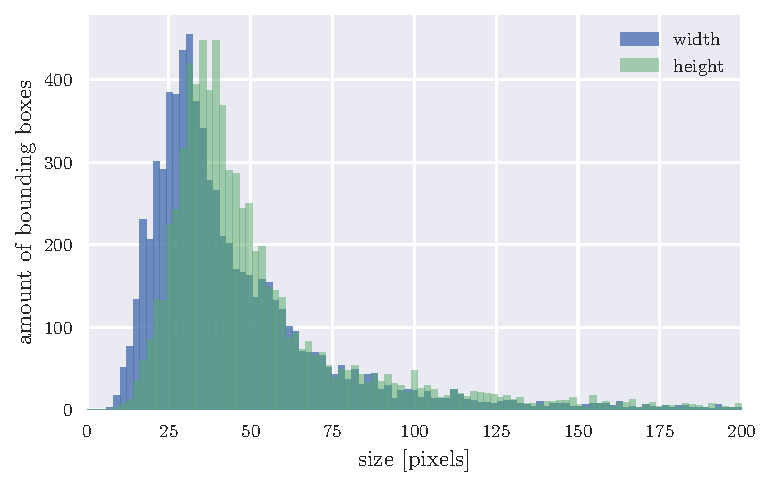
\includegraphics[width = 0.9\linewidth]{images/dataset_histogram.pdf}
    \caption{Histogram of bonding boxes dimensions in the dataset}
    \label{fig:hist_caries_dim}
\end{figure}

\begin{figure}
    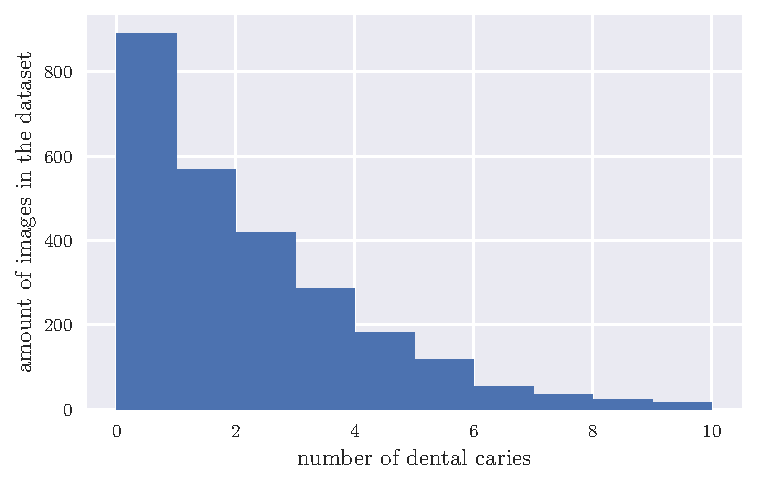
\includegraphics[width=0.9\linewidth]{images/caries_histogram.pdf}
    \caption{Histogram of the number of dental caries per image}
    \label{fig:hist_caries_per_img}
\end{figure}
\subsubsection{Image augmentations}

\subsubsection{Fifth stage}
\label{sec:dataset:fifth_stage}
In this stage, we finished the annotation of all 1400 images uploaded in stage four, resulting in 3989 X-rays with 7257 annotations. We plotted a histogram representing the distribution of the number of carries among images; it can be noticed in figure \ref{fig:hist_caries_per_img}.


\begin{table}
    \centering
    \begin{tabular}{|l|r|r|}
        \hline
                                       & Width [px] & Height [px] \\\hline
        Image size                     & 1068       & 795-847     \\ \hline
        Minimal box size               & 8          & 9           \\ \hline
        Maximal box size               & 384        & 315         \\ \hline
        Mean of box size               & 47.55      & 53.15       \\ \hline
        Standard deviation of box size & 37.99      & 35.33       \\ \hline
    \end{tabular}
    \caption{\label{tab:dataset_statistics}Statistics of bounding boxes, that denote position of carious lesions}
\end{table}

\subsubsection{Sixth stage}
\label{sec:dataset:sixth_stage}
We evaluated the model's performance on the test, validation, and training part of the dataset. Although the model used for prediction achieved $AP@.5 = 0.72$, there were 1598 images with at least one false positive or false negative detection. We decided that doing a second round of dataset review would be more beneficial than further expansion of the size of the dataset. We focused only on erroneous images and uploaded those 1598 images with no less than a single error to the CVAT annotation tool for review. When writing this thesis, there is still undergoing work on the uploaded images. Therefore, we were not able to use the sixth stage.


\section{Dental restorations}
\label{sec:dataset:dental_rotorations}
\begin{figure}
    \centering
    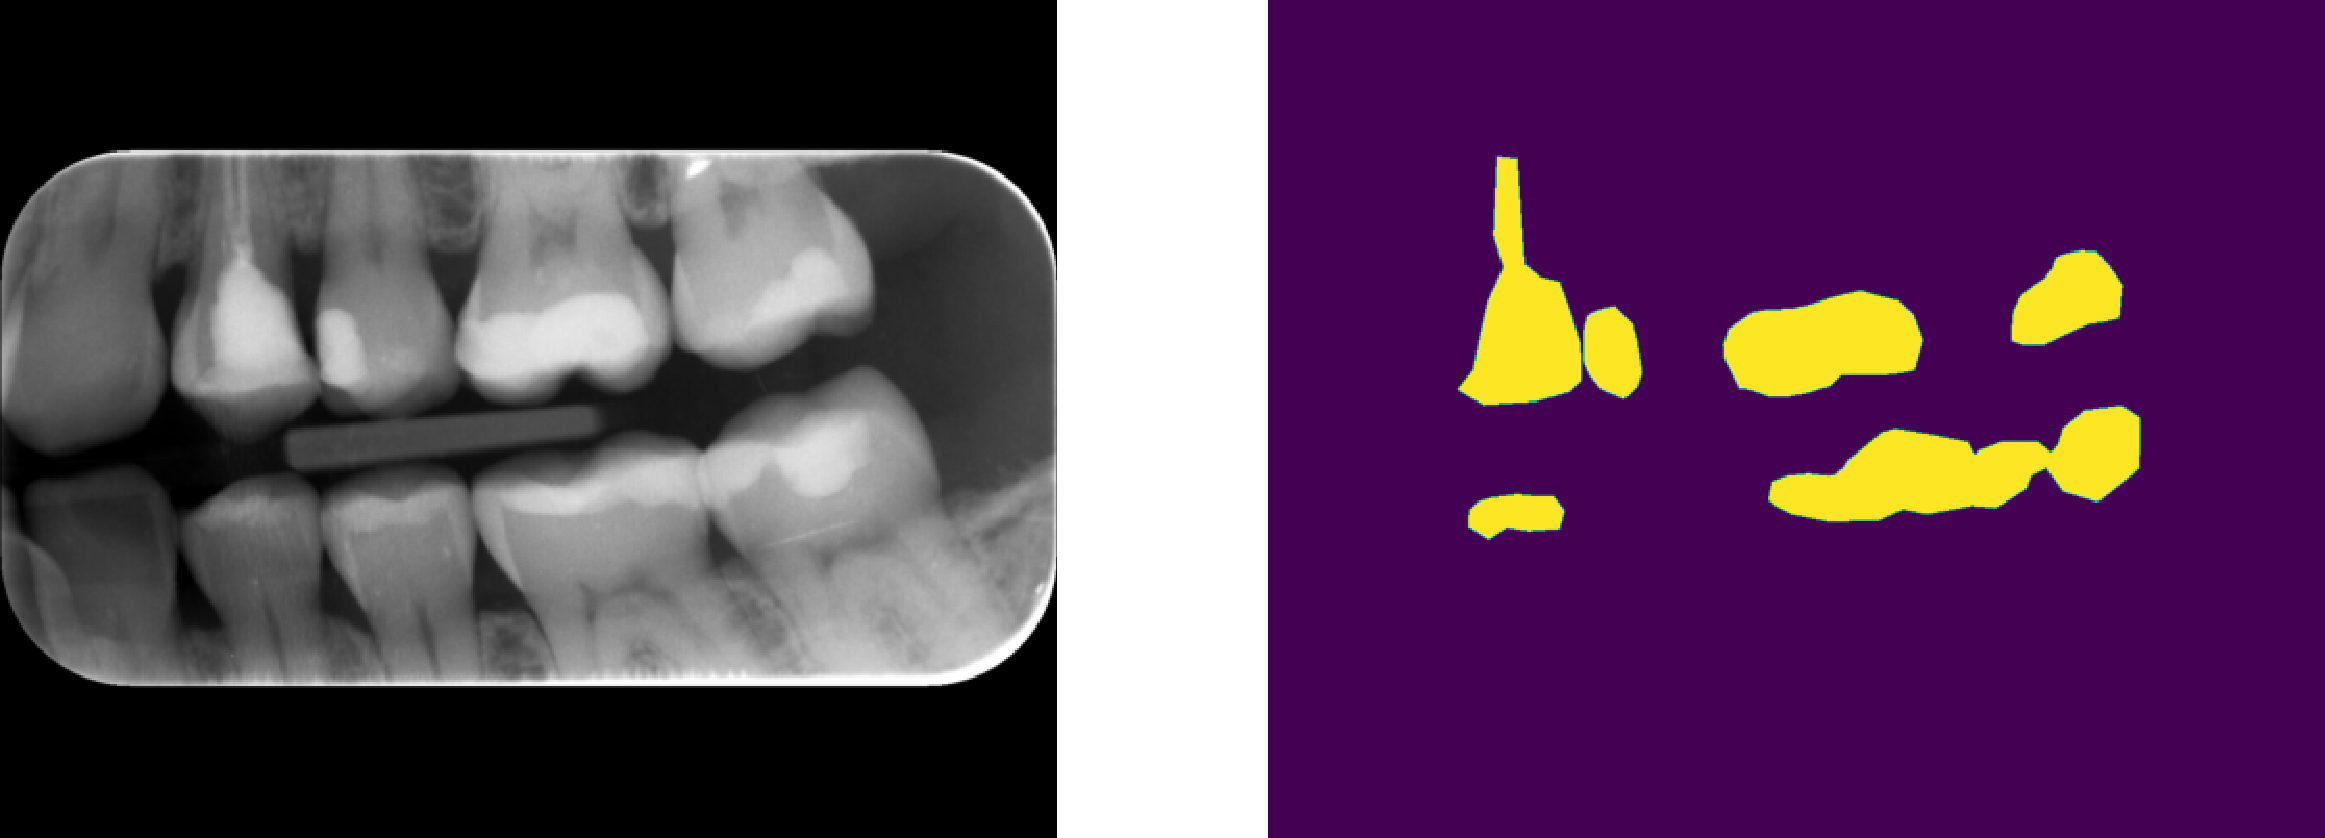
\includegraphics[width=\linewidth]{images/segmentation_ds_sample.pdf}
    \caption{Bitewing X-ray image on the left, pixel mask of the X-ray on the right (dental restorations have yellow color)}
    \label{fig:segmentation_sample}
\end{figure}
This dataset consists of a subset of images used in the dental caries dataset. MDDr. Tichy's team annotated it in the CVAT tool by drawing a polygon around each dental restoration. The work was done by the same group of dentistry students as stage one of the caries dataset and reviewed by a single fifth-year dentistry student. Evaluation of the whole dataset performed by a single person should ensure consistency among images. A total of 521 images were used to create this dataset, and an inspection revealed that 387 radiographs contained at least a single annotated restoration, and 134 had none.
The dataset was exported from CVAT in COCO format and saved on the CMP server. When working with the data, we used a pixel mask instead of polygons to denote the position of dental restorations. A sample of the dataset with a pixel mask is featured in figure \ref{fig:segmentation_sample}.

In figure \ref{fig:segmentation_restoration_size} we can  notice how many percent of the X-ray image consists of restorations. This gives us an idea of how common dental restorations in our data are. In figure \ref{fig:segmentation_patch_size} we see how the size of each restoration is distributed. Inspecting this figure, we observe that most restorations are smaller than $2\%$ of the image.

\begin{figure}
    \centering
    \begin{floatrow}[2]
        \ffigbox[\FBwidth]{\caption{Histogram of restoration area in image, images without restorations omited}\label{fig:segmentation_restoration_size}}%
        {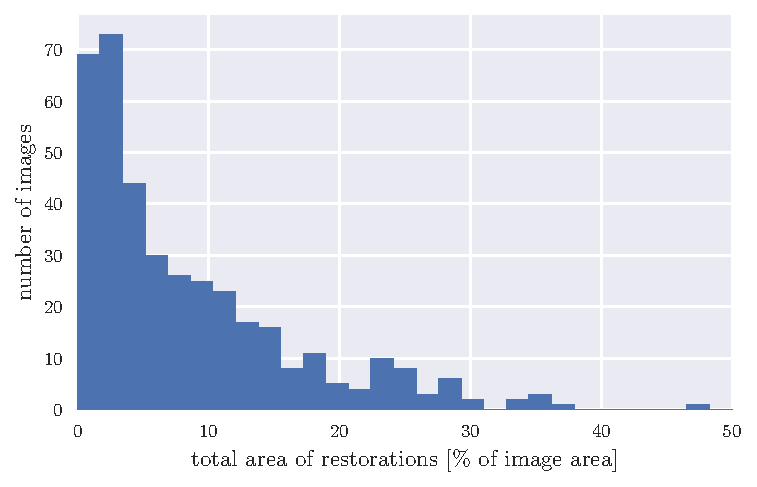
\includegraphics[width=\linewidth]{images/histogram_of_restoration_size.pdf}}\;
        \ffigbox[\FBwidth]{\caption{Histogram of areas of restorations, 10 largest omited}\label{fig:segmentation_patch_size}}
        {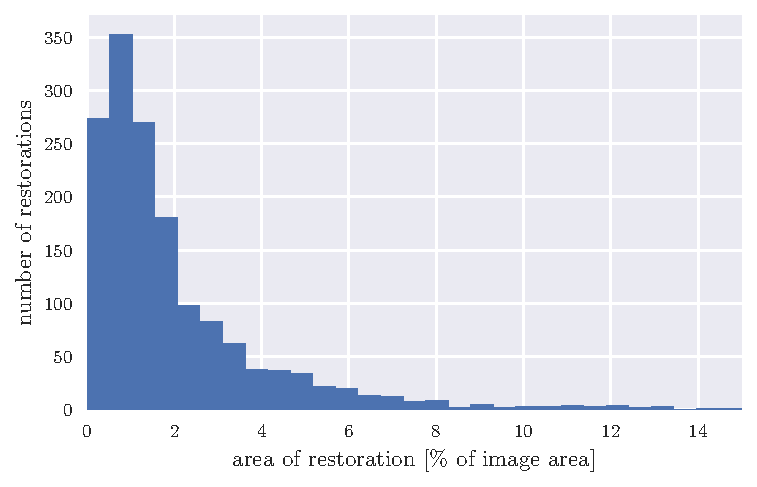
\includegraphics[width=\linewidth]{images/histogram_of_patch_size.pdf}}
    \end{floatrow}
\end{figure}